% The attention of the forecast head during training (Section "Forecast
% head"), for T_p = 4: one row per token of the sequence h_0..h_3, f_0..f_3.
% Each row shows the tokens that the bold token reads.
% Rows h_t: h_t reads h_0..h_t. Rows f_t: f_t reads h_0..h_t and f_0..f_t,
% and its output predicts patch t + 1. Build: pdflatex head_attention.tex
\documentclass[tikz,border=1pt]{standalone}
\usepackage[T1]{fontenc}
\usepackage{amsmath}
\usetikzlibrary{arrows.meta,calc}
\definecolor{clat}{HTML}{A2D6F3}   % encoder latent h: sky blue
\definecolor{cfor}{HTML}{F1CA73}   % forecast f: orange
\begin{document}
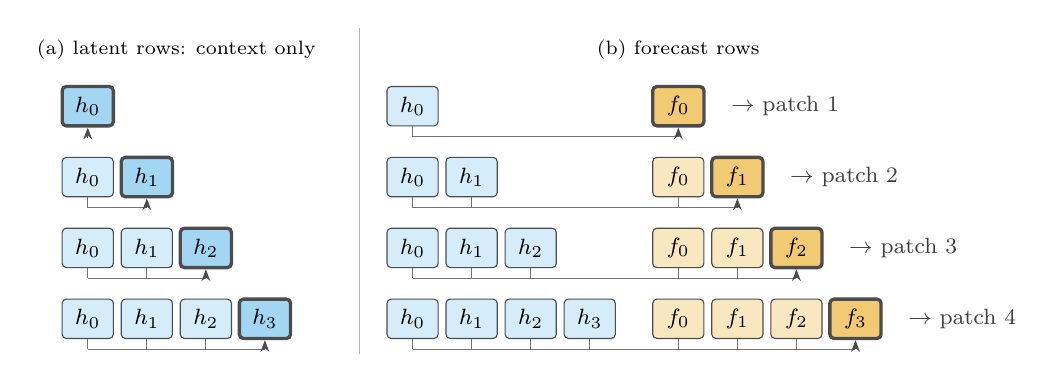
\begin{tikzpicture}[
  font=\footnotesize,
  tok/.style={draw=black!70, rounded corners=1.5pt, minimum width=6.5mm,
    minimum height=5mm, inner sep=1pt},
  arr/.style={-{Stealth[length=1.5mm]}, black!70},
  wire/.style={black!55},
]
  \def\dx{7.5mm}
  \def\dy{9mm}
  % Rows 0..3: the latent h_t reads h_0 .. h_t.
  \foreach \t in {0,...,3} {
    \pgfmathsetmacro{\y}{-\t*\dy}
    \foreach \j in {0,...,\t} {
      \ifnum\j<\t
        \node[tok, fill=clat!45] (a\t\j) at (\j*\dx, \y pt) {$h_{\j}$};
      \else
        \node[tok, fill=clat, very thick] (a\t\j) at (\j*\dx, \y pt) {$h_{\j}$};
      \fi
    }
    \coordinate (lo) at ($(a\t0.south) + (0, -1.3mm)$);
    \draw[wire] (lo) -- (lo -| a\t\t.south);
    \foreach \j in {0,...,\t} {
      \ifnum\j<\t \draw[wire] (a\t\j.south) -- (a\t\j.south |- lo); \fi
    }
    \draw[arr] (lo -| a\t\t.south) -- (a\t\t.south);
  }
  % Rows 4..7: the forecast f_t reads h_0 .. h_t and f_0 .. f_t.
  \foreach \t in {0,...,3} {
    \pgfmathsetmacro{\y}{-\t*\dy}
    \foreach \j in {0,...,\t}
      \node[tok, fill=clat!45] (h\t\j) at ({(\j + 5.5)*\dx}, \y pt) {$h_{\j}$};
    \foreach \j in {0,...,\t} {
      \pgfmathsetmacro{\x}{(\j + 10)*\dx}
      \ifnum\j<\t
        \node[tok, fill=cfor!45] (f\t\j) at (\x pt, \y pt) {$f_{\j}$};
      \else
        \node[tok, fill=cfor, very thick] (f\t\j) at (\x pt, \y pt) {$f_{\j}$};
      \fi
    }
    \coordinate (lo) at ($(h\t0.south) + (0, -1.3mm)$);
    \draw[wire] (lo) -- (lo -| f\t\t.south);
    \foreach \j in {0,...,\t} {
      \draw[wire] (h\t\j.south) -- (h\t\j.south |- lo);
      \ifnum\j<\t \draw[wire] (f\t\j.south) -- (f\t\j.south |- lo); \fi
    }
    \draw[arr] (lo -| f\t\t.south) -- (f\t\t.south);
    \node[anchor=west, text=black!75] at ($(f\t\t.east) + (2mm, 0)$)
      {$\to$ patch $\pgfmathparse{int(\t+1)}\pgfmathresult$};
  }
  % Column labels.
  \node[font=\scriptsize] at (1.5*\dx, 0.8*\dy)
    {(a) latent rows: context only};
  \node[font=\scriptsize] at (10*\dx, 0.8*\dy)
    {(b) forecast rows};
  \draw[black!30] (4.6*\dx, 1.1*\dy) -- (4.6*\dx, -3.5*\dy);
\end{tikzpicture}
\end{document}
